\chapter{Multi-Agent Systems}
\label{appx-b:multi-agent-systems}

This appendix, Appendix~\ref{appx-b:multi-agent-systems}, presents additional details on the MAS implementation.
More specifically, the method used to implement FIPA are presented, and the main communication protocols that war used within this method are detailed.

\section{FIPA Implementation}

\nomenclature[G]{JADE}{JAVA Agent Communication Language}
\nomenclature[G]{ACL}{Agent Communication Language}

The Foundation for Intelligent Physical Agents (FIPA) has established a standard set of protocols that allow agents to interact with each other.
These protocols form the so called Agent Communication Language (ACL)
Telecom Italia has successively begun to develop a JAVA Agent Development Framework (JADE) that puts the entire ACL at the programmer's disposal.
Published under LGPL (i.e. the Lesser General Public License Version 2), JADE is a free software package that can easily be used to construct large MASs.

In order to perform optimisation functions however, a way to interact with OpenDSS was required.
On Microsoft Windows, the ActiveX COM server provided a simple access point to MATLAB and OpenDSS specific functions, and the JAVA COM Bridge (JACOB) made this server accessible to the JAVA run-time environment.

JADE and JACOB were, respectively, obtained from the following two sources:

\begin{itemize}
	\item JADE: \textit{http://jade.tilab.com}
	\item JACOB: \textit{https://sourceforge.net/projects/jacob-project/}
\end{itemize}

By including the \textit{jade.jar} and \textit{jacob.jar}, and the corresponding Dynamic Linked Libraries (DLLs) \textit{jacob-1.8-M2-x86.dll} and  \textit{jacob-1.8-M2-x64.dll}, FIPA was fully implemented and linked to MATLAB and OpenDSS.

\section{Communication Protocols}

The main three protocols that were used within Chapter~\ref{ch3} are:

\begin{enumerate}
	\item FIPA Query Protocol (FIPA-standard-SC00027H)
	\item FIPA Brokering Protocol (FIPA-standard-SC00033H)
	\item FIPA ContractNet Protocol (FIPA-standard-SC00029H)
\end{enumerate}

The flowcharts for these three protocols were taken from the corresponding standards and, for completeness, are explained in the following three subsections.

\subsection{FIPA Query Protocol}
\label{appx-b:subsec:fipa-query-protocol}

\begin{figure}\centering
	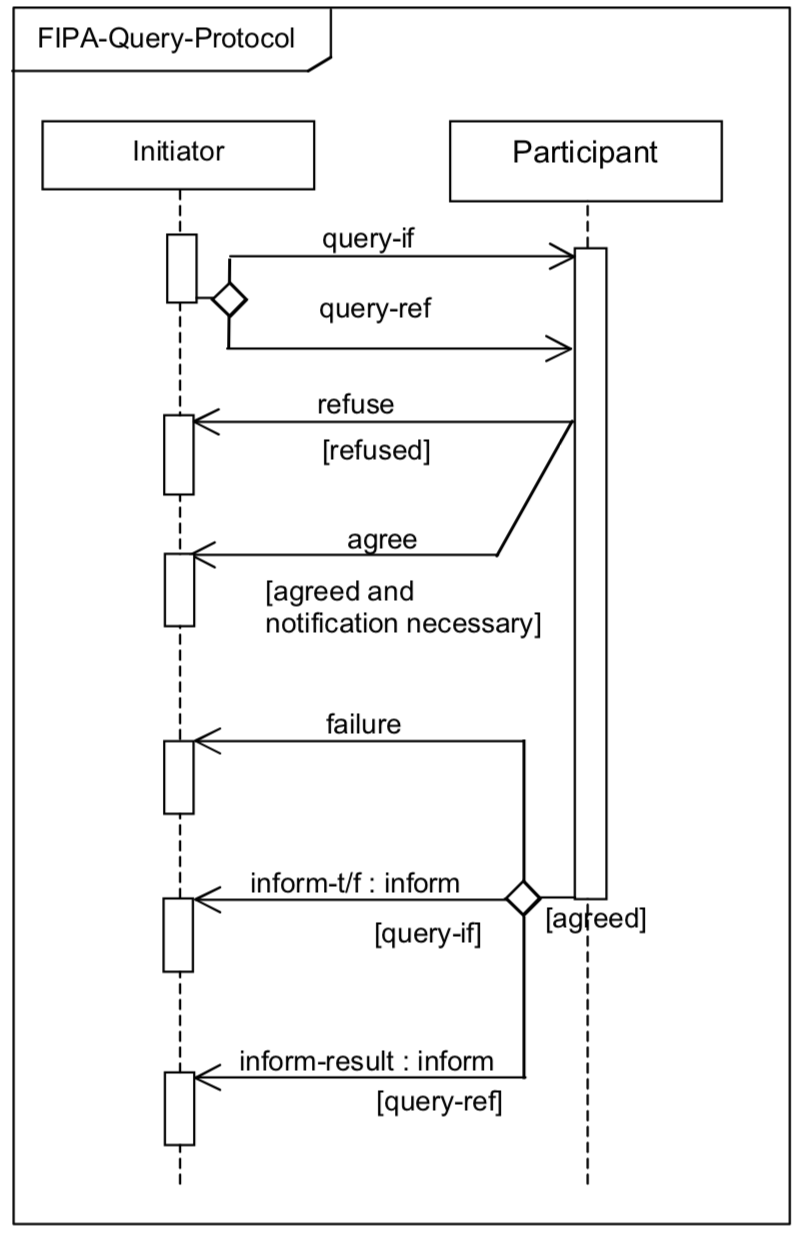
\includegraphics[width=0.5\linewidth]{_appendices/_a2/fig/fipa-query}
	\caption{FIPA Query Protocol flow chart}
	\label{appx-b:fig:fipa-query}
\end{figure}

Figure~\ref{appx-b:fig:fipa-query} shows the complete flow chart of the FIPA Query protocol.
This protocol is initiated by an ``\textit{initiator}'' that send a ``\textit{query}'' message (either ``if'' or ``reference'' message) to a ``\textit{Participant}''.
In Chapter~\ref{ch3}, the initiators were the brokering agents of the loads and the participant were the brokering agents of the energy supplier.
The \textit{participant} replies either with an ``\textit{agree}'' to inform the \textit{initiator} that the query is received, or a ``\textit{refuse}'' message is sent to terminate the communication.
After an \textit{agree} message, the \textit{participant} sends the required information in an ``\textit{inform}'' message (as a reply to the ``if'' or ``reference'' query), or a ``\textit{failure}'' is sent when no data is available.
In Chapter~\ref{ch3}, the data that is sent in the \textit{inform} messages includes the daily load profile onto which the EV agents should superimpose their charging demand.

\subsection{FIPA Brokering protocol}
\label{appx-b:subsec:fipa-brokering-protocol}

\begin{figure}\centering
	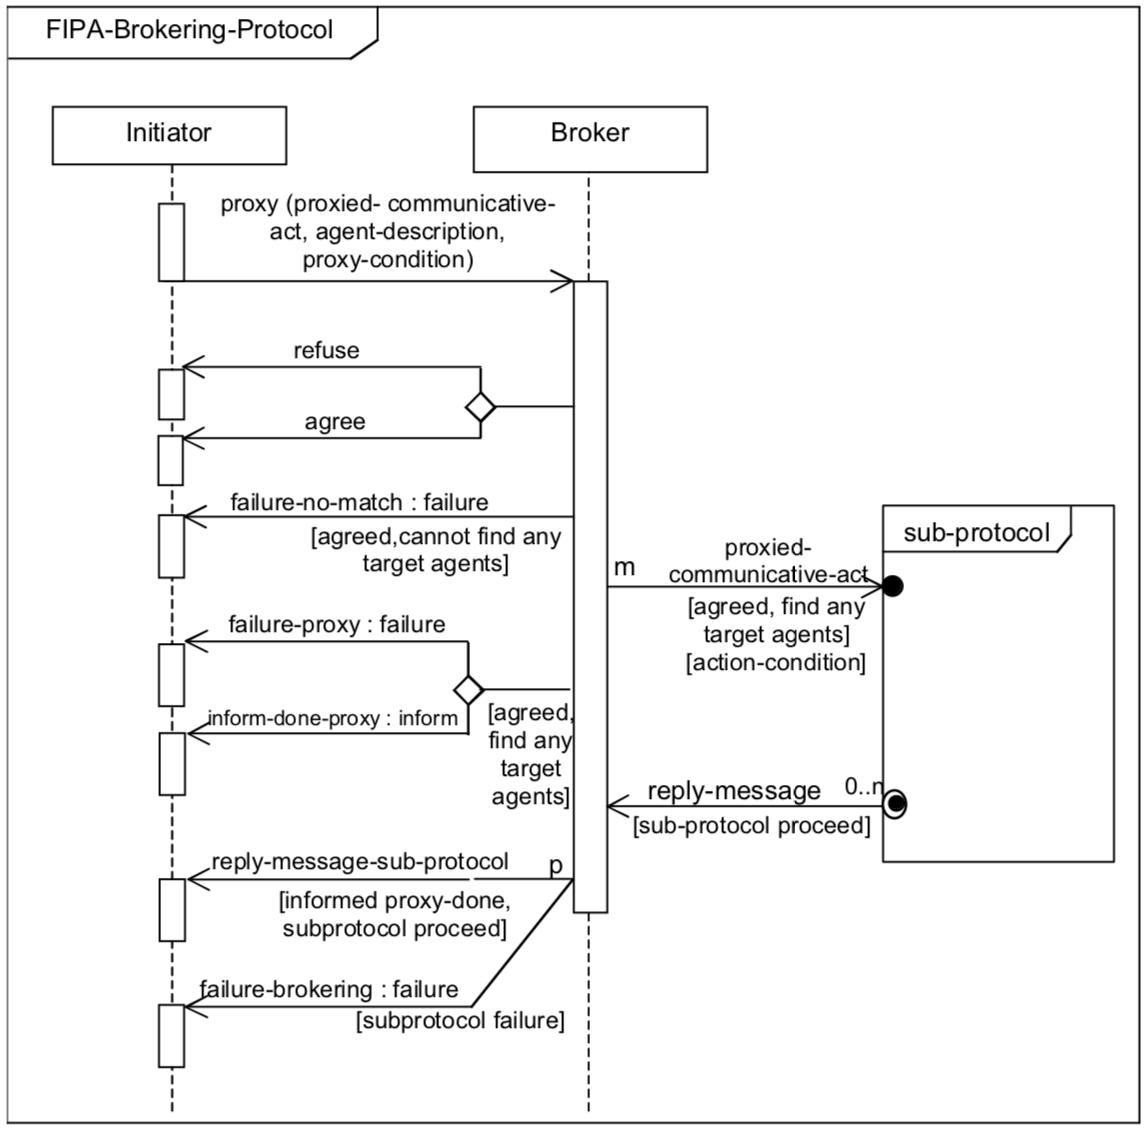
\includegraphics[width=0.66\linewidth]{_appendices/_a2/fig/fipa-brokering}
	\caption{FIPA Brokering Protocol flow chart}
	\label{appx-b:fig:fipa-brokering}
\end{figure}

The brokering protocol, as shown in Figure~\ref{appx-b:fig:fipa-brokering}, is used to delegate an agents task to a different agent in order to free up its own computational resources.
In Chapter~\ref{ch3} for instance, the load agents never communicate with the energy supplier directly, since the applying and undoing of power profiles is delegated to their brokering agents.
The protocol is initiated by assigning a broker to a load agent by sending a ``\textit{proxy}'' message.
This message contains the required information for the broker, like the power profile a buying broker should apply.
If the broker can fulfil this request, then an ``\textit{agree}'' message is sent, otherwise a ``\textit{refuse}'' message is sent.
The broker uses the FIPA Query protocol, as explained in Section~\ref{appx-b:subsec:fipa-query-protocol}, to obtain a list of broker agents that are linked to energy suppliers, which can be used to apply the load's demand profile.
However, if no such broker is found, then a ``\textit{failure}'' (i.e. ``no match'') message is sent.
Alternatively, the broker begins its delegating task and it forwards the requested demand profile to the corresponding energy supplier (i.e. it uses the FIPA ContractNet protocol as outlined in the next section, Section~\ref{appx-b:subsec:fipa-contract-net-protocol}).
If an error occurs during this delegating process, then a ``\textit{failure}'' message is sent (i.e. ``proxy failure'' or ``inform falure'').
Upon successful delegation, the broker replies to the ``\textit{Initiator}'' with a ``\textit{reply}'' message that contains information about the applied demand profile.
Theoretically, this information can also contain pricing information, yet this feature was disregarded since it lies outside the scope of this thesis.

\subsection{FIPA ContractNet Protocol}
\label{appx-b:subsec:fipa-contract-net-protocol}

\begin{figure}\centering
	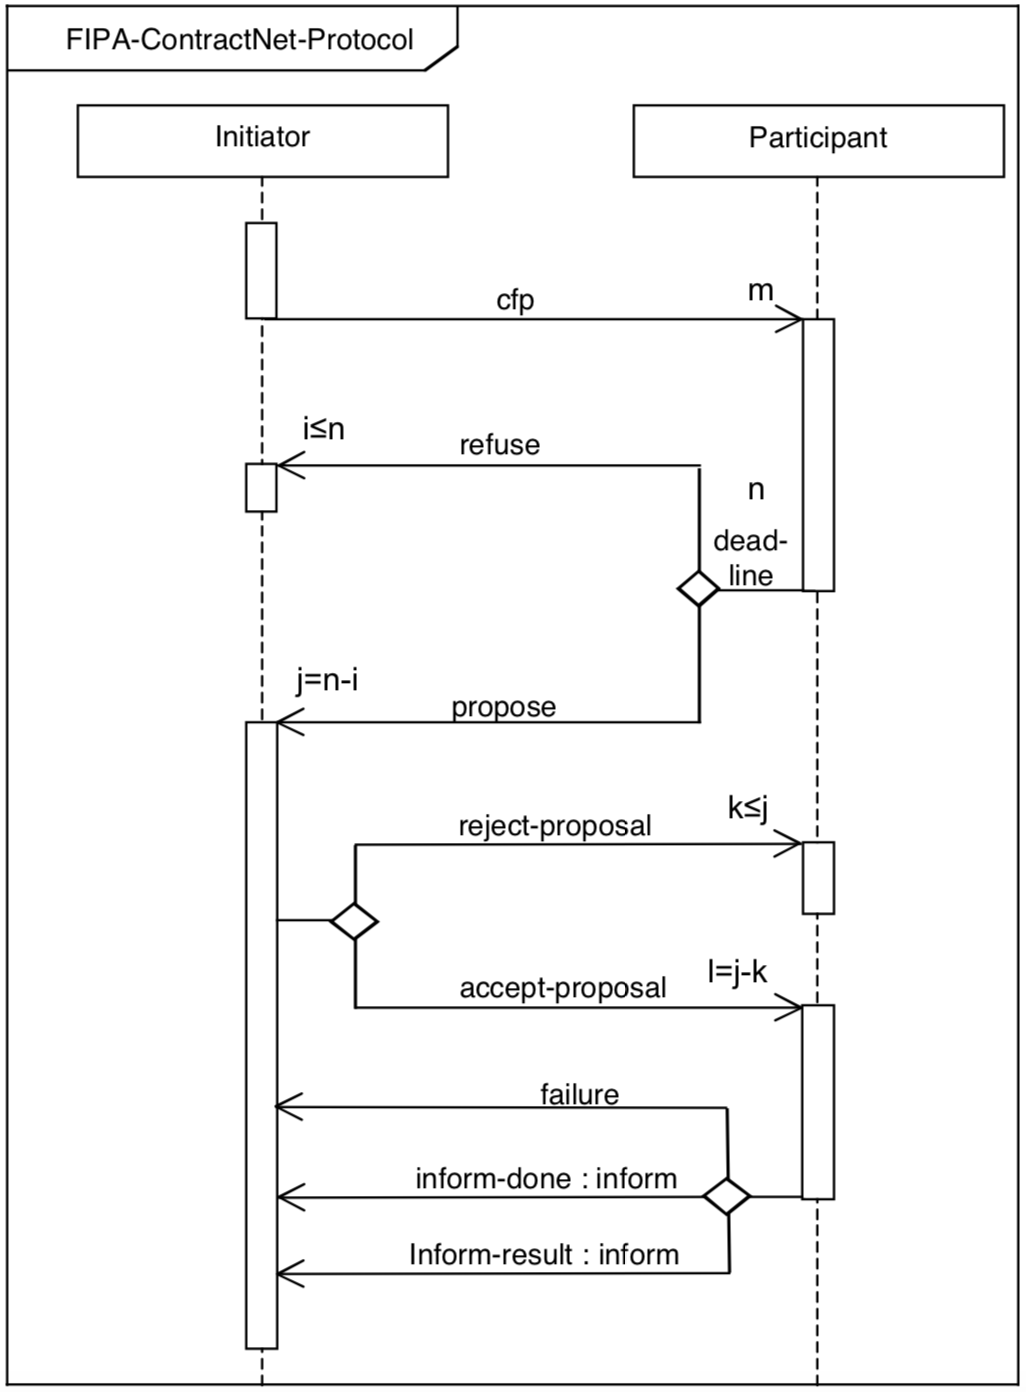
\includegraphics[width=0.5\linewidth]{_appendices/_a2/fig/fipa-contract-net}
	\caption{FIPA ContractNet Protocol flow chart}
	\label{appx-b:fig:fipa-contract-net}
\end{figure}

Figure~\ref{appx-b:fig:fipa-contract-net} shows the FIPA ContractNet Protocol that allows an agent to negotiate a binding contract.
After executing this dual handshake protocol, all contract participants are informed about the final contract decision and no information is lost during the message exchange.
The protocol is initiated by an ``\textit{Initiator}'', who sends a ``\textit{Call For Proposal}'' (\textit{cfp}) to $m$ ``\textit{Participant}s''.
This \textit{cfp} contains a deadline within which all agents that do want to participate should reply.
They can reject their participation by sending a ``\textit{refuse}'' message, or acknowledge their participation by sending a ``\textit{propose}'' message that also contains proposition information (for example pricing information).
Once all participants have replied or the deadline has expired, the \textit{initiator} continues executing.
It collects and assesses all proposals, choses the accepted and rejected ones and, respectively, issues ``\textit{accept}'' and ``\textit{reject}'' notifications.
The participating agents reply with an ``\textit{inform}'' message if they acknowledge the ``accept`` or ``reject'' message, and in case of an error, they reply with a ``failure'' message.






